\documentclass[12pt,a4paper]{article}

\usepackage[a4paper,margin=2.35cm]{geometry}
\usepackage{fontspec}
\usepackage{graphicx}
\usepackage{booktabs}
\usepackage{tabularx}
\usepackage{array}
\usepackage{longtable}
\usepackage{float}
\usepackage{caption}
\usepackage{subcaption}
\usepackage{xcolor}
\usepackage{hyperref}
\usepackage{enumitem}
\usepackage{microtype}
\usepackage{listings}
\usepackage{xspace}

\setmainfont{Arial}
\setsansfont{Arial}
\setmonofont{Consolas}
\hypersetup{
  colorlinks=true,
  linkcolor=blue!50!black,
  urlcolor=blue!50!black,
  citecolor=blue!50!black
}
\captionsetup{font=small,labelfont=bf}
\renewcommand{\figurename}{Hình}
\renewcommand{\tablename}{Bảng}
\renewcommand{\abstractname}{Tóm tắt}
\setlist[itemize]{leftmargin=1.4em,itemsep=0.15em}
\setlist[enumerate]{leftmargin=1.6em,itemsep=0.15em}
\lstset{
  basicstyle=\ttfamily\footnotesize,
  breaklines=true,
  frame=single,
  columns=fullflexible,
  keepspaces=true,
  backgroundcolor=\color{gray!6}
}

\newcommand{\code}[1]{\texttt{#1}}
\newcommand{\shape}{\code{10000x10000x10000}\xspace}

\title{\textbf{Báo cáo thực nghiệm song song hóa phép nhân ma trận lớn bằng C và Open MPI}}
\author{Nhóm thực hiện: [Điền tên nhóm]}
\date{Tháng 6 năm 2026}

\begin{document}
\maketitle
\thispagestyle{empty}

\begin{abstract}
Báo cáo trình bày quá trình xây dựng và thực nghiệm chương trình nhân ma trận kích thước lớn bằng ngôn ngữ C và Open MPI trên cụm 3 máy Windows Subsystem for Linux (WSL). Từ yêu cầu ban đầu là nhân ma trận vuông, chương trình đã được mở rộng thành phép nhân ma trận chữ nhật tổng quát $A(M \times K) \times B(K \times N) = C(M \times N)$, dữ liệu đầu vào là số nguyên ngẫu nhiên trong đoạn $[0,1000]$ nhưng lưu bằng kiểu \code{double}. Trọng tâm thực nghiệm là biến thể \code{mpi\_2d}, lấy ý tưởng từ cách chia lưới 2 chiều: mỗi tiến trình nhận một block hàng của $A$, một block cột của $B$ đã transpose, sau đó tính block cục bộ của $C$.

Với bài toán chính \shape, tổng số phép toán xấp xỉ $2 \times 10^{12}$ FLOP. Thực nghiệm quét số tiến trình trên 3 node cho thấy cấu hình 9 tiến trình cho thời gian tốt nhất 144.972 giây, đạt 13.796 GFLOP/s. Cấu hình 12 tiến trình đứng thứ hai với 148.039 giây, chỉ chậm hơn khoảng 2.12\%. Các cấu hình dùng nhiều tiến trình hơn như 16, 25, 36 và 44 lại chậm hơn do chi phí pack/send tập trung tại rank 0 và số thông điệp MPI tăng nhanh. Kết quả checksum của tất cả cấu hình đều trùng nhau, chứng minh khác biệt thời gian đến từ hiệu năng chứ không phải sai lệch kết quả tính toán.
\end{abstract}

\newpage

\section{Giới thiệu và cơ sở lý thuyết}
Nhân ma trận là một phép toán nền tảng trong tính toán hiệu năng cao, xuất hiện trong mô phỏng khoa học, xử lý ảnh, đồ họa, học máy và nhiều bài toán đại số tuyến tính. Với phép nhân $A(M \times K) \times B(K \times N)$, mỗi phần tử $C_{ij}$ được tính bằng:
\[
  C_{ij} = \sum_{t=0}^{K-1} A_{it}B_{tj}.
\]
Độ phức tạp tính toán là $O(MKN)$, còn số phép toán dấu phẩy động thường được ước lượng là $2MKN$ vì mỗi cặp nhân-cộng tương ứng hai FLOP.

Khi $M=K=N=10000$, riêng số phần tử của mỗi ma trận vuông đã là 100 triệu. Nếu lưu bằng \code{double}, mỗi ma trận cần khoảng 800 MB, còn ba ma trận đầy đủ cần khoảng 2.4 GB chưa tính buffer MPI, buffer pack và overhead hệ thống. Quan trọng hơn, tổng số phép toán là $2 \times 10^{12}$ FLOP. Vì vậy, chạy tuần tự không còn phù hợp cho mục tiêu thực nghiệm trong thời gian ngắn; chương trình cần song song hóa để phân phối khối lượng tính toán cho nhiều core và nhiều máy.

Mục tiêu của đề tài gồm bốn điểm chính:
\begin{enumerate}
  \item Xây dựng chương trình C/Open MPI có thể nhân ma trận lớn với kích thước tổng quát $M,K,N$.
  \item Cài đặt nhiều biến thể để so sánh: tuần tự, tiled, MPI chia hàng và MPI chia lưới 2D.
  \item Thiết lập cụm nhiều máy WSL trong cùng mạng LAN để chạy thực nghiệm thật.
  \item Đo thời gian, thông lượng, checksum và phân tích vì sao một số cấu hình tiến trình nhanh hơn cấu hình khác.
\end{enumerate}

Báo cáo này tập trung vào kết quả cuối cùng của quá trình thực nghiệm: benchmark chính bằng biến thể \code{mpi\_2d} trên 3 node với các cấu hình 4, 9, 12, 16, 25, 36 và 44 tiến trình MPI.

\section{Thiết kế chương trình}
\subsection{Mô hình dữ liệu}
Phiên bản cuối của chương trình sử dụng mô hình tổng quát:
\[
  A(M \times K) \times B(K \times N) = C(M \times N).
\]
Người dùng nhập kích thước qua CLI bằng \code{--m M --k K --n N}. Cách đặt tên này tránh nhầm lẫn với phiên bản cũ, trong đó \code{--n} từng được hiểu là ma trận vuông $N \times N$. Ở phiên bản mới, \code{--n} là số cột của ma trận kết quả.

Dữ liệu đầu vào được sinh ngẫu nhiên xác định theo seed, stream và index. Giá trị thực chất là số nguyên trong $[0,1000]$ nhưng lưu bằng \code{double}. Cách làm này giữ được tính dễ kiểm chứng của checksum, đồng thời không làm thay đổi cấu trúc thuật toán nhân ma trận dấu phẩy động.

\subsection{Các biến thể thuật toán}
Chương trình có các biến thể chính sau:
\begin{itemize}
  \item \code{seq}: nhân ma trận tuần tự theo ba vòng lặp chuẩn.
  \item \code{seq\_tiled}: phiên bản tuần tự có chia tile để cải thiện locality của cache.
  \item \code{mpi}: chia hàng của $A$ cho các tiến trình, broadcast toàn bộ $B$, mỗi rank tính một dải hàng của $C$.
  \item \code{mpi\_tiled}: tương tự \code{mpi}, nhưng local multiply dùng tile.
  \item \code{mpi\_2d}: chia tiến trình theo lưới 2D, mỗi rank xử lý một block con của $C$.
\end{itemize}

Trong các benchmark lớn, báo cáo tập trung vào \code{mpi\_2d} vì biến thể này phù hợp hơn với ý tưởng chia khối 2 chiều của file \code{matrix-v2.cpp}: thay vì mỗi rank chỉ nhận một dải hàng, các rank được đặt lên lưới $(row\_parts, col\_parts)$; mỗi rank nhận một block hàng của $A$ và một block cột của $B$.

\subsection{Luồng tính của \code{mpi\_2d}}
Với $P$ tiến trình, chương trình chọn layout 2D từ các ước số của $P$ theo mục tiêu cân bằng lưới và phù hợp tỉ lệ $M/N$, cùng tinh thần với \code{MPI\_Dims\_create}. Trên benchmark vuông, log và bảng tổng hợp xác nhận $P=9$ dùng layout $3 \times 3$, $P=12$ dùng $3 \times 4$ và $P=44$ dùng $4 \times 11$. Block $B$ được pack ở dạng transpose để vòng lặp local đọc liên tục theo bộ nhớ.

Pseudo-code rút gọn của luồng \code{mpi\_2d}:
\begin{lstlisting}
if rank == 0:
    generate A, B from seed
    layout = choose_2d_layout(P, M, N)
    for each rank r:
        pack A rows for grid_row(r)
        pack B columns for grid_col(r) as B_local_T
        send A_local and B_local_T to r

each rank:
    compute C_local from A_local and B_local_T
    checksum_local = checksum(C_local)

reduce checksum_local to rank 0
\end{lstlisting}

Điểm đáng chú ý là việc pack/send hiện vẫn tập trung ở rank 0. Thiết kế này dễ giải thích, sát với mục tiêu giáo dục và thuận tiện đối chiếu checksum, nhưng nó cũng tạo ra bottleneck khi số tiến trình tăng quá cao: số block và số thông điệp tăng gần theo $P$, còn rank 0 phải điều phối tuần tự nhiều phần dữ liệu hơn.

\section{Môi trường thực nghiệm}
\subsection{Cụm máy}
Thực nghiệm cuối được chạy trên 3 máy WSL trong cùng mạng LAN. Tổng số logical core sẵn có là 44. Cấu hình nhận diện trong quá trình chạy như sau:
\begin{table}[H]
\centering
\caption{Cấu hình cụm máy dùng trong benchmark cuối}
\begin{tabularx}{\textwidth}{lrlX}
\toprule
Node & Logical core & Định danh node & Vai trò \\
\midrule
node1 & 12 & node1 & Master, rank khởi chạy Open MPI \\
node2 & 16 & node2 & Worker \\
node3 & 16 & node3 & Worker \\
\bottomrule
\end{tabularx}
\end{table}

Các node dùng Open MPI qua SSH/TCP. Do chạy trong WSL, script chạy có cấu hình thêm wrapper SSH để tắt các biến môi trường đồ họa như \code{DISPLAY} và giới hạn một số component HWLOC không cần thiết. Điều này giúp tránh treo hoặc chậm do WSLg/OpenGL khi Open MPI dò topology.

\subsection{Cấu hình hostfile}
Các hostfile được tạo để ép số slot theo từng thí nghiệm. Ví dụ, cấu hình 9 tiến trình chia đều 3 tiến trình trên mỗi node:
\begin{lstlisting}
node1 slots=3
node2 slots=3
node3 slots=3
\end{lstlisting}

Cấu hình 44 tiến trình dùng toàn bộ logical core hiện có:
\begin{lstlisting}
node1 slots=12
node2 slots=16
node3 slots=16
\end{lstlisting}

Việc ép slot rõ ràng rất quan trọng, vì mục tiêu không chỉ là chạy được chương trình mà còn biết chính xác mỗi node đang đóng góp bao nhiêu tiến trình.

\section{Phương pháp đo}
\subsection{Bài toán benchmark}
Bài toán chính là:
\[
  A(10000 \times 10000) \times B(10000 \times 10000) = C(10000 \times 10000).
\]
Các tham số cố định:
\begin{itemize}
  \item Variant: \code{mpi\_2d}.
  \item Shape: \shape.
  \item Seed: \code{2026}.
  \item Tile/panel: \code{10000}.
  \item Số node: 3.
  \item Không lưu full matrix kết quả để tránh overhead I/O không cần thiết.
\end{itemize}

Lệnh chạy có dạng:
\begin{lstlisting}
mpirun <MPI_FLAGS> --hostfile config/hosts_P -np P ./build/matrix_hpc \
  --variant mpi_2d \
  --m 10000 --k 10000 --n 10000 \
  --repeat 1 --tile 10000 --seed 2026 \
  --max-ram-gb 7 \
  --output-dir outputs/report_10000 \
  --checksum-file results/report_10000_process_sweep_checksums.csv \
  --run-label report_10000_process_sweep \
  --mapping slots_... --pe 1
\end{lstlisting}

Thời gian benchmark được lấy trong phần chạy song song MPI, tức sau khi chương trình đã vào luồng MPI và không tính các thao tác ngoài phạm vi thực nghiệm như thao tác shell hay chuẩn bị thủ công từ Windows.

\subsection{Chỉ số đánh giá}
Các chỉ số chính:
\begin{itemize}
  \item \textbf{Runtime}: thời gian chạy tính bằng giây.
  \item \textbf{GFLOP/s}: thông lượng, tính theo công thức $\frac{2MKN}{time \times 10^9}$.
  \item \textbf{Checksum}: hash và tổng kiểm tra của ma trận kết quả, dùng để xác nhận các cấu hình cho cùng kết quả.
  \item \textbf{Speedup tương đối}: trong báo cáo này dùng mốc p4 vì không chạy tuần tự cho benchmark chính trong thực nghiệm cuối.
\end{itemize}

Do p9 và p16 được chạy lặp lại 3 lần, bảng kết quả có cả thời gian trung bình và độ lệch chuẩn. Các cấu hình khác được chạy 1 lần để hoàn tất sweep trên dữ liệu rất lớn trong thời gian hợp lý.

\section{Kết quả thực nghiệm}
\subsection{Bảng tổng hợp}
\begin{table}[H]
\centering
\caption{Kết quả benchmark chính với \code{mpi\_2d}}
\small
\begin{tabular}{rrrrrrrl}
\toprule
P & Grid & Runs & Min (s) & Avg (s) & Std (s) & Best GFLOP/s & Mapping \\
\midrule
4  & $2\times2$  & 1 & 172.477 & 172.477 & 0.000 & 11.596 & \code{2/1/1} \\
9  & $3\times3$  & 3 & 144.972 & 152.407 & 8.710 & 13.796 & \code{3/3/3} \\
12 & $3\times4$  & 1 & 148.039 & 148.039 & 0.000 & 13.510 & \code{4/4/4} \\
16 & $4\times4$  & 3 & 189.611 & 193.133 & 4.345 & 10.548 & \code{4/6/6} \\
25 & $5\times5$  & 1 & 214.462 & 214.462 & 0.000 & 9.326 & \code{7/9/9} \\
36 & $6\times6$  & 1 & 255.644 & 255.644 & 0.000 & 7.823 & \code{10/13/13} \\
44 & $4\times11$ & 1 & 304.251 & 304.251 & 0.000 & 6.574 & \code{12/16/16} \\
\bottomrule
\end{tabular}
\end{table}

Trong các cấu hình đã đo, p9 có best/min runtime tốt nhất với thời gian 144.972 giây. p12 đứng thứ hai với 148.039 giây, chậm hơn khoảng:
\[
  \frac{148.039 - 144.972}{144.972} \times 100 \approx 2.12\%.
\]
So với p16 tốt nhất, p9 nhanh hơn khoảng:
\[
  \frac{189.611 - 144.972}{189.611} \times 100 \approx 23.54\%.
\]

\subsection{Biểu đồ thời gian và thông lượng}
\begin{figure}[H]
\centering
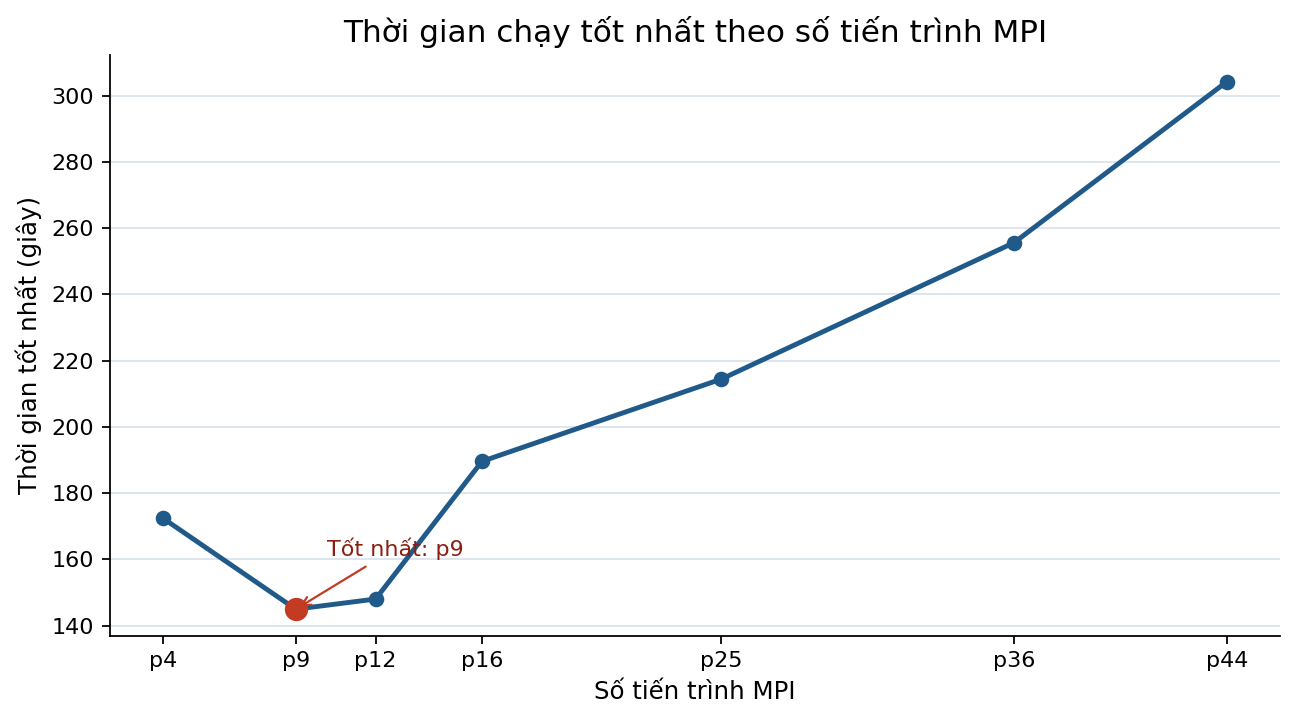
\includegraphics[width=0.93\textwidth]{figures/runtime_by_process.png}
\caption{Thời gian chạy tốt nhất theo số tiến trình MPI. p9 cho runtime thấp nhất, p12 rất gần, còn p16 trở lên chậm dần.}
\end{figure}

\begin{figure}[H]
\centering
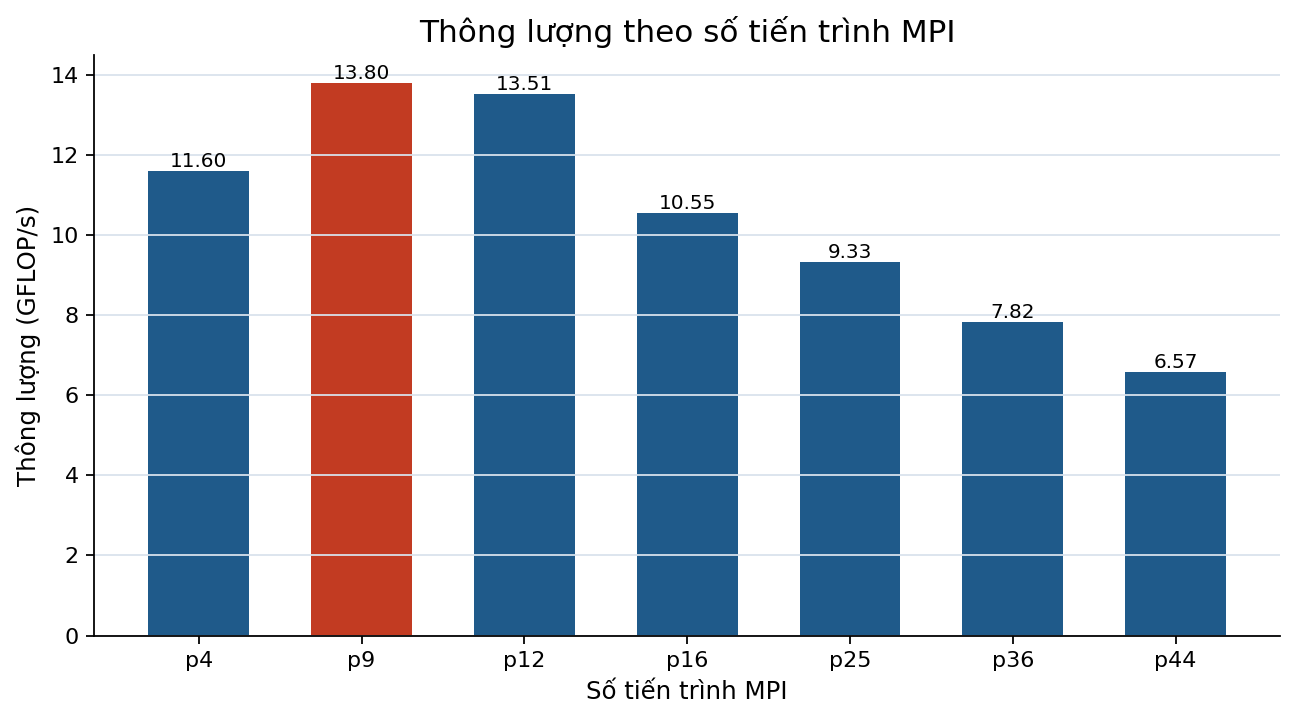
\includegraphics[width=0.93\textwidth]{figures/gflops_by_process.png}
\caption{Thông lượng GFLOP/s theo số tiến trình. Cấu hình p9 đạt đỉnh 13.796 GFLOP/s.}
\end{figure}

\subsection{Speedup tương đối và hiệu suất}
Vì benchmark chính quá lớn để chạy tuần tự trong khung thời gian thực nghiệm, báo cáo dùng p4 làm mốc tương đối. Đây không phải speedup tuyệt đối so với tuần tự, nhưng vẫn cho thấy xu hướng mở rộng khi tăng số tiến trình.

\begin{figure}[H]
\centering
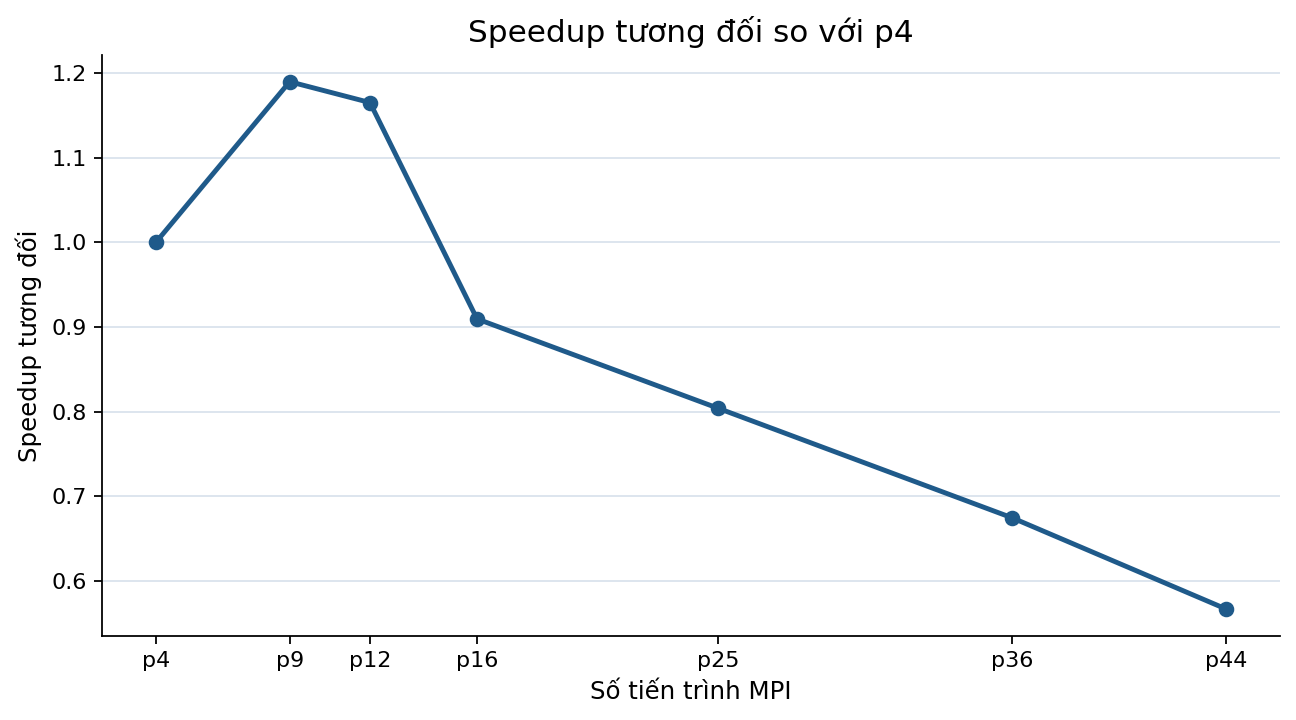
\includegraphics[width=0.93\textwidth]{figures/speedup_vs_p4.png}
\caption{Speedup tương đối so với p4. Đây là chỉ số scaling tương đối, không phải speedup chuẩn $T(1)/T(p)$ của đề bài vì không chạy được bản tuần tự trong khung thời gian thực nghiệm.}
\end{figure}

\begin{figure}[H]
\centering
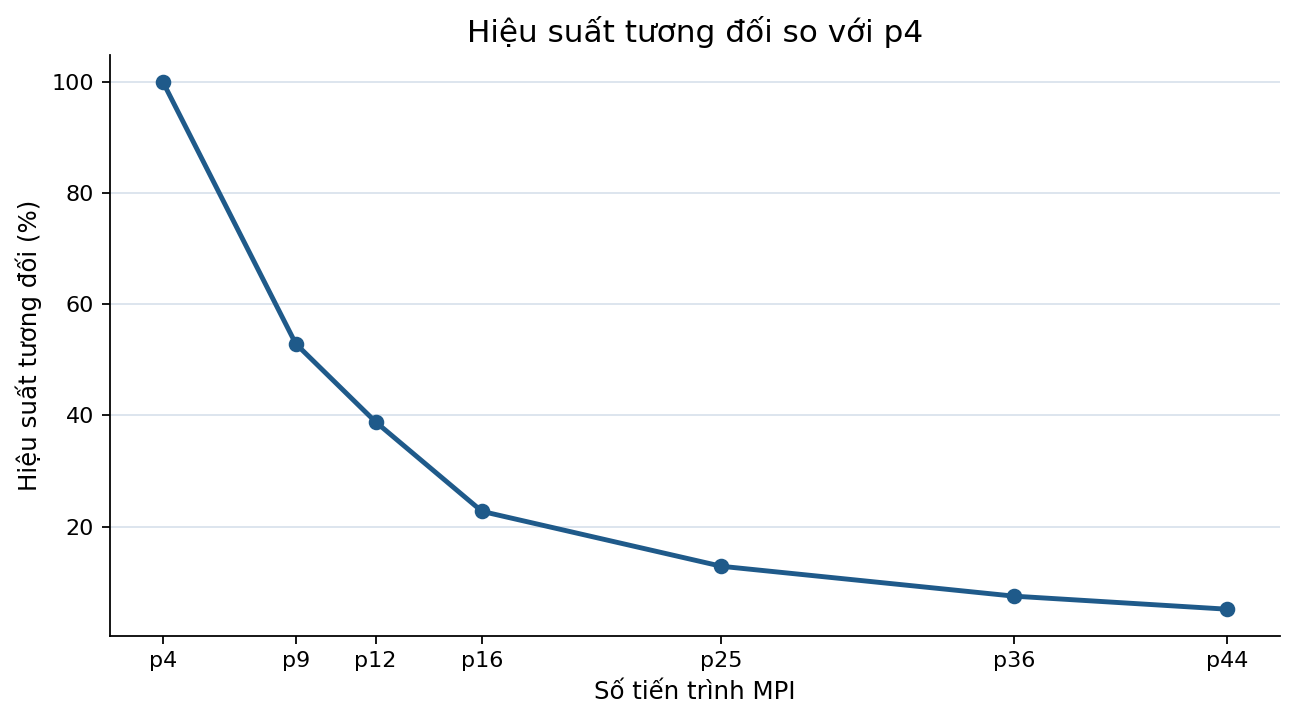
\includegraphics[width=0.93\textwidth]{figures/efficiency_vs_p4.png}
\caption{Hiệu suất tương đối so với p4. Hiệu suất giảm mạnh khi số tiến trình tăng vì chi phí giao tiếp và phân phối dữ liệu tăng nhanh hơn lợi ích tính toán.}
\end{figure}

\subsection{Kiểm tra tính đúng}
Tất cả cấu hình trong sweep đều có cùng checksum hash:
\[
  \code{c14405814301863a}.
\]
Điều này chứng minh chương trình tính nhất quán trên các layout 2D khác nhau. Bảng checksum summary ghi nhận mỗi cấu hình chỉ có một checksum duy nhất và trạng thái \code{OK}. Vì vậy, khác biệt runtime không đến từ việc bỏ sót rank, sai mapping hoặc sai dữ liệu đầu vào.

\section{Phân tích kết quả}
\subsection{Vì sao p9 có best runtime tốt nhất?}
Kết quả p9 có best/min runtime tốt nhất trong sweep ban đầu có thể gây bất ngờ, vì cụm có 44 logical core và trực giác thường là ``nhiều core hơn sẽ nhanh hơn''. Tuy nhiên, với implementation hiện tại, giới hạn không nằm hoàn toàn ở năng lực tính toán cục bộ. Giới hạn lớn nằm ở rank 0: rank này phải pack block $A$, pack block $B$ đã transpose và gửi buffer cho từng rank.

Khi tăng số tiến trình, mỗi rank tính ít hơn, nhưng:
\begin{itemize}
  \item số block cần phân phối tăng;
  \item số thông điệp MPI tăng;
  \item tổng dữ liệu pack/send từ rank 0 có thể tăng theo layout;
  \item rank 0 trở thành điểm nghẽn trước khi các worker được sử dụng hiệu quả.
\end{itemize}

Với p9, layout là $3 \times 3$, mỗi node chạy 3 tiến trình. Cấu hình này đủ song song để giảm đáng kể khối lượng tính trên mỗi rank, nhưng chưa tạo quá nhiều block và thông điệp. Với p12, layout $3 \times 4$ vẫn còn hợp lý nên kết quả rất gần p9. Từ p16 trở lên, overhead phân phối bắt đầu lớn hơn lợi ích tăng thêm từ compute.

\subsection{Vì sao p44 không nhanh nhất?}
p44 dùng toàn bộ logical core của cụm: 12 tiến trình trên node1, 16 trên node2 và 16 trên node3. Layout 2D thực tế của p44 là $4 \times 11$, tức \code{row\_parts}=4 và \code{col\_parts}=11. Vì số phần chia cột là 11, block cột của $B$ nhiều hơn, số buffer cần pack nhiều hơn và số lần gửi tăng lên rõ rệt.

Trong lý tưởng, nếu dữ liệu đã phân tán sẵn và thuật toán dùng broadcast/scatter theo communicator hàng-cột như Cannon, SUMMA hoặc một biến thể collective 2D đầy đủ, p44 có thể tận dụng nhiều core tốt hơn. Nhưng với code hiện tại, việc rank 0 tự pack và gửi tuần tự làm p44 phải trả chi phí điều phối quá lớn. Kết quả thực nghiệm phản ánh đúng giới hạn thiết kế: p44 đạt 304.251 giây, chậm hơn hơn 2 lần so với p9.

\subsection{Ý nghĩa của p12}
Theo yêu cầu kiểm tra thêm, p12 đã được chạy sau khi nghi ngờ p9 có thể chưa phải điểm tốt nhất. Kết quả p12 là 148.039 giây, chỉ chậm hơn p9 khoảng 2.12\%. Điều này cho thấy p12 cũng là một cấu hình rất tốt để báo cáo. Tuy nhiên, p9 chạy 3 lần còn p12 mới chạy 1 lần, nên không nên diễn giải quá mức rằng p9 chắc chắn tốt hơn p12 trong mọi lần chạy. Để kết luận ổn định hơn giữa p9 và p12, nên chạy lặp p12 nhiều lần trong điều kiện mạng tương tự.

Diễn giải hợp lý là p9 và p12 nằm gần điểm cân bằng của hệ thống: đủ tiến trình để khai thác cả 3 node, nhưng chưa vượt qua ngưỡng overhead giao tiếp. Khi số tiến trình vượt ngưỡng này, bottleneck ở rank 0 làm hiệu năng giảm.

\section{Đánh giá thiết kế hiện tại}
\subsection{Ưu điểm}
Thiết kế hiện tại có một số ưu điểm rõ:
\begin{itemize}
  \item Hỗ trợ ma trận chữ nhật tổng quát, không bị giới hạn ở ma trận vuông.
  \item Dữ liệu random deterministic nên có thể so sánh checksum giữa các variant và giữa các lần chạy.
  \item \code{mpi\_2d} thể hiện được ý tưởng chia lưới 2 chiều, gần với hướng tiếp cận trong \code{matrix-v2.cpp}.
  \item Với benchmark lớn, chương trình tránh gather full $C$ khi không cần thiết, giảm bộ nhớ và I/O.
  \item Script benchmark ghi lại mapping, process count, checksum, runtime và GFLOP/s, phù hợp cho báo cáo thực nghiệm.
\end{itemize}

\subsection{Hạn chế}
Hạn chế quan trọng nhất là cơ chế phân phối dữ liệu còn tập trung. Rank 0 vừa sinh dữ liệu, vừa pack, vừa gửi block cho mọi rank. Với số tiến trình nhỏ đến trung bình, chi phí này chấp nhận được. Nhưng khi p tăng lên 25, 36 hoặc 44, chi phí điều phối tăng nhanh và làm mất lợi ích của việc có thêm core.

Ngoài ra, cụm chạy trên WSL và Wi-Fi/LAN dân dụng nên không thể so với một cluster HPC thật có mạng InfiniBand, filesystem dùng chung và topology ổn định. Điều này không làm mất giá trị thực nghiệm, nhưng cần được nêu rõ để tránh diễn giải quá mức.

Benchmark chính tập trung vào quét số process trên 3 node vì đây là kịch bản dữ liệu lớn ổn định nhất nhóm hoàn tất được. Báo cáo chưa có sweep đầy đủ 1 node, 2 node và 3 node trên cùng một shape lớn; đây là phần nên bổ sung nếu môi trường mạng ổn định hơn.

\subsection{Hướng tối ưu tiếp theo}
Nếu tiếp tục tối ưu, các hướng có giá trị nhất là:
\begin{enumerate}
  \item Thay rank 0 send tuần tự bằng collective phù hợp hơn, ví dụ scatter theo communicator hàng/cột.
  \item Triển khai thuật toán kiểu SUMMA: chia $K$ theo panel, broadcast panel $A$ theo hàng process và panel $B$ theo cột process.
  \item Dùng non-blocking MPI như \code{MPI\_Isend}/\code{MPI\_Irecv} để overlap giao tiếp với tính toán.
  \item Sinh dữ liệu phân tán trực tiếp trên từng rank dựa vào seed và global index, giảm nhu cầu rank 0 giữ và pack toàn bộ đầu vào.
  \item Tối ưu kernel local bằng blocking sâu hơn hoặc BLAS nếu mục tiêu chuyển từ giáo dục sang hiệu năng cao thực sự.
\end{enumerate}

Trong phạm vi đề tài, phiên bản hiện tại có ưu điểm là rõ ràng, dễ demo và có số liệu chứng minh. Các hướng trên phù hợp để đưa vào phần phát triển tiếp theo.

\section{Đối chiếu yêu cầu đề bài}
\begin{table}[H]
\centering
\caption{Mức đáp ứng các yêu cầu chính của đề bài}
\small
\begin{tabularx}{\textwidth}{lX}
\toprule
Yêu cầu & Minh chứng trong bài làm \\
\midrule
Chương trình tuần tự & Có \code{seq} và \code{seq\_tiled}, dùng cùng bộ sinh dữ liệu và checksum. \\
Cơ sở lý thuyết và độ phức tạp & Có công thức $C_{ij}$, độ phức tạp $O(MKN)$ và ước lượng $2MKN$ FLOP. \\
Chương trình song song MPI & Có \code{mpi}, \code{mpi\_tiled} và \code{mpi\_2d}. \\
Dữ liệu kích thước lớn & Benchmark chính, tương ứng $2\times10^{12}$ FLOP. \\
Thay đổi số process & Đã đo p4, p9, p12, p16, p25, p36 và p44 trên 3 node. \\
Thay đổi số node & Benchmark chính chạy trên 3 node; sweep 1/2/3 node đầy đủ được nêu là hạn chế thực nghiệm. \\
Execution time và GFLOP/s & Có bảng runtime, thông lượng và biểu đồ tương ứng. \\
Speedup/Efficiency & Đáp ứng một phần: có speedup/efficiency tương đối theo p4; chưa có speedup chuẩn $T(1)/T(p)$ cho benchmark chính. \\
Tính đúng & Tất cả cấu hình benchmark chính có cùng checksum hash \code{c14405814301863a}. \\
\bottomrule
\end{tabularx}
\end{table}

\section{Kết luận}
Đề tài đã xây dựng được chương trình nhân ma trận lớn bằng C và Open MPI, hỗ trợ phép nhân tổng quát $A(M \times K) \times B(K \times N)$ với các biến thể tuần tự, tiled, MPI chia hàng và \code{mpi\_2d}. Tất cả cấu hình benchmark chính đều cho cùng checksum hash \code{c14405814301863a}, xác nhận tính đúng và tính tái lập của kết quả.

Trên benchmark chính với $2 \times 10^{12}$ FLOP, p9 có best/min runtime tốt nhất trong các cấu hình đã đo: 144.972 giây và 13.796 GFLOP/s. p12 rất gần p9 với 148.039 giây, chỉ chậm hơn 2.12\%, nhưng p12 mới chạy 1 lần nên cần lặp thêm trong điều kiện mạng tương tự để kết luận ổn định hơn. p16, p25, p36 và p44 chậm hơn do bottleneck pack/send tập trung tại rank 0. Vì vậy, muốn p44 hoặc cấu hình nhiều tiến trình hơn thật sự tốt hơn, cần chuyển sang cơ chế phân phối dữ liệu phi tập trung hơn, ví dụ SUMMA hoặc broadcast panel theo communicator 2D.

\newpage
\appendix
\section{Phụ lục: dữ liệu nguồn}
Dữ liệu tổng hợp dùng trong báo cáo được lấy từ các file:
\begin{itemize}
  \item \code{results/report\_10000\_process\_sweep\_raw.csv}
  \item \code{results/report\_10000\_process\_sweep\_summary.csv}
  \item \code{results/report\_10000\_process\_sweep\_checksum\_summary.csv}
  \item \code{results/report\_10000\_final\_process\_sweep.md}
\end{itemize}

\section{Phụ lục: lệnh kiểm tra mapping p9}
Để xác nhận p9 thật sự dùng cả 3 node với 3 tiến trình mỗi node, lệnh kiểm tra hostname được chạy qua Open MPI và kết quả có dạng:
\begin{lstlisting}
3 BangPC
3 DESKTOP-A3I1NIN
3 LAPTOP-34RTNCDV
\end{lstlisting}

Điều này loại trừ khả năng p9 chỉ chạy trên một hoặc hai máy.

\section{Phụ lục: thử nghiệm mở rộng 15000 và 20000}
Sau benchmark chính, nhóm kiểm tra thêm khả năng chạy dữ liệu lớn hơn. Cluster 3 node vẫn qua smoke test Open MPI và chạy được bài nhỏ trên 3 node. Tuy nhiên, các thử nghiệm \code{20000x20000x20000} và \code{15000x15000x15000} trên WSL/LAN bị dừng bởi lỗi Open MPI TCP timeout dạng \code{mca\_btl\_tcp\_frag\_recv: readv failed: Connection timed out}. Vì các run này không sinh dòng \code{RESULT} và không có checksum hoàn tất, báo cáo không dùng chúng làm kết quả hiệu năng chính. Chúng được ghi nhận như giới hạn của môi trường thử nghiệm WSL qua mạng LAN dân dụng, không phải lỗi tính toán của thuật toán.

\section{Tài liệu tham khảo}
\begin{itemize}
  \item Open MPI Project. \textit{Open MPI Documentation}. \url{https://docs.open-mpi.org/}
  \item Open MPI Project. \textit{MPI\_Dims\_create manual page}. \url{https://docs.open-mpi.org/en/v5.0.3/man-openmpi/man3/MPI_Dims_create.3.html}
  \item Robert A. van de Geijn và Jerrell Watts. \textit{SUMMA: Scalable Universal Matrix Multiplication Algorithm}. Netlib LAPACK Working Note 96. \url{https://www.netlib.org/lapack/lawnspdf/lawn96.pdf}
  \item AMATH 483/583 High-Performance Scientific Computing. \textit{Lecture 20: Cannon's Algorithm}. \url{https://amath583.github.io/sp22/units/L20.html}
  \item Đề bài báo cáo cuối kỳ học phần Tính toán hiệu năng cao, 2026.
\end{itemize}

\end{document}
